\documentclass[11pt]{article}
\usepackage[a4paper,margin=1in,top=0.85in,bottom=0.9in]{geometry}
\usepackage[T1]{fontenc}
\usepackage[utf8]{inputenc}
\usepackage{lmodern}
\usepackage{microtype}
\usepackage{hyperref}
\usepackage{xcolor}
\usepackage{colortbl}
\usepackage{listings}
\usepackage{longtable}
\usepackage{booktabs}
\usepackage{graphicx}
\usepackage{tabularx}
\usepackage{array}
\usepackage[most]{tcolorbox}
\usepackage{fancyhdr}
\usepackage{titlesec}
\usepackage{enumitem}
\usepackage{float}
\usepackage{caption}

% ---------------------------------------------------------------------------
% Color palette
% ---------------------------------------------------------------------------
\definecolor{primary}{HTML}{1A3A5C}
\definecolor{accent}{HTML}{2E86AB}
\definecolor{tableheader}{HTML}{1A3A5C}
\definecolor{tablealt}{HTML}{EEF4FA}
\definecolor{highlight}{HTML}{E8F4FD}
\definecolor{finding}{HTML}{FFFBEB}
\definecolor{findingrule}{HTML}{D97706}
\definecolor{okgreen}{HTML}{16A34A}
\definecolor{warnred}{HTML}{DC2626}
\definecolor{codebg}{HTML}{F8F9FA}

% ---------------------------------------------------------------------------
% Section heading style
% ---------------------------------------------------------------------------
\titleformat{\section}
  {\color{primary}\Large\bfseries}{\thesection}{1em}{}
  [\color{accent}\vspace{2pt}\titlerule\vspace{4pt}]
\titleformat{\subsection}
  {\color{primary}\large\bfseries}{\thesubsection}{1em}{}
\titleformat{\subsubsection}
  {\color{accent}\normalsize\bfseries}{\thesubsubsection}{1em}{}

% ---------------------------------------------------------------------------
% Page header / footer
% ---------------------------------------------------------------------------
\pagestyle{fancy}
\fancyhf{}
\fancyhead[L]{\color{primary}\small DS503 \textbf{Project 2} -- Advanced Hadoop}
\fancyhead[R]{\color{primary}\small Patadia $\cdot$ V.\,Patel $\cdot$ N.\,Patel}
\fancyfoot[C]{\color{primary}\small\thepage}
\renewcommand{\headrulewidth}{0.4pt}
\renewcommand{\footrulewidth}{0pt}

% ---------------------------------------------------------------------------
% Column types
% ---------------------------------------------------------------------------
\newcolumntype{Y}{>{\raggedright\arraybackslash}X}
% Colored header cell (left-aligned)
\newcolumntype{H}{>{\columncolor{tableheader}\color{white}\bfseries}l}

% ---------------------------------------------------------------------------
% tcolorbox styles
% ---------------------------------------------------------------------------
\tcbset{
  finding/.style={
    colback=finding, colframe=findingrule,
    boxrule=0.5pt, left=8pt, right=8pt, top=5pt, bottom=5pt,
    fonttitle=\bfseries\small, title={Key Finding}
  },
  note/.style={
    colback=highlight, colframe=accent,
    boxrule=0.5pt, left=8pt, right=8pt, top=5pt, bottom=5pt,
    fonttitle=\bfseries\small
  }
}

% ---------------------------------------------------------------------------
% Listings style
% ---------------------------------------------------------------------------
\lstdefinestyle{code}{
  basicstyle=\ttfamily\small,
  breaklines=true,
  frame=single,
  backgroundcolor=\color{codebg},
  rulecolor=\color{accent!40},
  columns=fullflexible
}

% ---------------------------------------------------------------------------
% Hyperref
% ---------------------------------------------------------------------------
\hypersetup{colorlinks=true, linkcolor=accent, urlcolor=accent, citecolor=accent}

% ---------------------------------------------------------------------------
% Helpers
% ---------------------------------------------------------------------------
% Colored table header row (use inside tabular/longtable)
\newcommand{\theadrow}[1]{%
  \rowcolor{tableheader}\color{white}\bfseries #1}

\title{%
  \color{primary}\bfseries DS503 Project 2 -- Advanced Hadoop\\[6pt]
  \large\color{accent} K-Means Clustering with Apache Pig \& Hadoop MapReduce%
}
\author{Shyam Patadia \and Vansh Patel \and Nischal Patel}
\date{\today}

% ===========================================================================
\begin{document}
\maketitle
\thispagestyle{fancy}

% ===========================================================================
\section{Implementation Coverage}
% ===========================================================================

\begin{longtable}{@{}p{0.22\linewidth}p{0.10\linewidth}p{0.60\linewidth}@{}}
  \rowcolor{tableheader}
  \color{white}\textbf{Requirement} &
  \color{white}\textbf{Done?} &
  \color{white}\textbf{Evidence} \\
  \midrule\endhead
  Task 1 (A--H in Pig)       & \textcolor{okgreen}{\textbf{Yes}} & \texttt{src/main/java/circlenet/taskA/taskA.pig} $\cdots$ \texttt{taskH/taskH.pig} \\
  \rowcolor{tablealt}
  Task 2.2(a)                & \textcolor{okgreen}{\textbf{Yes}} & \texttt{single\_k5\_r1/summary.txt} \\
  Task 2.2(b)                & \textcolor{okgreen}{\textbf{Yes}} & \texttt{basic\_k5\_r10/summary.txt} \\
  \rowcolor{tablealt}
  Task 2.2(c)                & \textcolor{okgreen}{\textbf{Yes}} & \texttt{early\_k5\_r30/summary.txt} \\
  Task 2.2(d)                & \textcolor{okgreen}{\textbf{Yes}} & \texttt{opt\_centers\_k5\_r30/summary.txt} (\texttt{used\_combiner=true}) \\
  \rowcolor{tablealt}
  Task 2.2(e)(i)             & \textcolor{okgreen}{\textbf{Yes}} & \texttt{opt\_centers\_k5\_r30/final\_centers.csv} + \texttt{summary.txt} (convergence flag) \\
  Task 2.2(e)(ii)            & \textcolor{okgreen}{\textbf{Yes}} & \texttt{opt\_points\_k5\_r30/final\_points\_with\_centers} \\
  \rowcolor{tablealt}
  Task 2.2(f)                & \textcolor{okgreen}{\textbf{Yes}} & K/R runtime tables, SSE tables, and qualitative analysis in Task 2 section \\
  Task 3(a) BYOD             & \textcolor{okgreen}{\textbf{Yes}} & \texttt{task3a\_byod\_poker\_artifacts/\ldots} \\
  \rowcolor{tablealt}
  Task 3(d) Visualization    & \textcolor{okgreen}{\textbf{Yes}} & \texttt{task3d\_viz\_output/\ldots}, \texttt{task3d\_viz\_py/out\_k*/\ldots} (synthetic 4D dataset from Task 2) \\
\end{longtable}

% ===========================================================================
\section{Task 1: Pig Implementation}
% ===========================================================================

For Project 2 Task 1, we rewrote Project 1 analytics Tasks A--H in Apache Pig and tested them on the same CircleNet dataset from Project 1. The Pig scripts are placed inside the same task folders as the original Java MapReduce code:

\begin{center}\small
\texttt{src/main/java/circlenet/task\{A--H\}/task\{A--H\}.pig}
\end{center}

We recorded Pig runtimes in \texttt{pig\_task\_times.csv} and compared them against the best MapReduce timings from Project 1 using \texttt{mr\_vs\_pig\_comparison.csv}.

% ---------------------------------------------------------------------------
\subsection{Implementation Summary by Task (A--H)}
% ---------------------------------------------------------------------------

\subsubsection*{Task A -- Frequency of FavoriteHobby}

\textbf{Pig idea:} Load pages, keep hobby field, group by hobby, count.

\textbf{Implementation:}
\begin{itemize}[noitemsep,topsep=2pt]
  \item Loaded CircleNetPage with full schema.
  \item Created a cleaned hobby relation using \texttt{TRIM(\ldots)} and removed null/empty values.
  \item Grouped by hobby and counted rows in each group.
\end{itemize}

\textbf{Design rationale:} Direct aggregation task. Pig handles it naturally with \texttt{GROUP + COUNT}, requiring no join or multi-stage logic.

\subsubsection*{Task B -- Top 10 Most Accessed Pages}

\textbf{Pig idea:} Count accesses per page, join with page metadata, sort descending, limit 10.

\textbf{Implementation:}
\begin{itemize}[noitemsep,topsep=2pt]
  \item Loaded ActivityLog and counted \texttt{whatpage} frequency.
  \item Joined counts with CircleNetPage (ID, nickname, job title).
  \item Ordered by access count descending and applied \texttt{LIMIT 10}.
\end{itemize}

\textbf{Design rationale:} Task requires both aggregation and a join. Pig relational operators make this concise; in MapReduce it required two separate jobs or a distributed cache.

\subsubsection*{Task C -- Users with a Chosen Hobby}

\textbf{Pig idea:} Filter only; no group, no join.

\textbf{Implementation:}
\begin{itemize}[noitemsep,topsep=2pt]
  \item Loaded pages.
  \item Filtered by hobby parameter \texttt{\$HOBBY} (case-insensitive \texttt{LOWER} compare).
  \item Projected only nickname and jobtitle.
\end{itemize}

\textbf{Design rationale:} In MapReduce this was implemented as a map-only job. The Pig script mirrors that design -- filter/projection only, no explicit reduce-style grouping stage.

\subsubsection*{Task D -- Popularity Factor (followers per owner, including zero)}

\textbf{Pig idea:} Compute follower counts by followed user (ID2), then left-outer-join with all page owners.

\textbf{Implementation:}
\begin{itemize}[noitemsep,topsep=2pt]
  \item Built owner list from CircleNetPage.
  \item Grouped follows by \texttt{id2} and counted followers.
  \item Left-outer joined owners with counts; replaced null with zero.
\end{itemize}

\textbf{Design rationale:} Keeps all owners including those with no followers, and avoids the single-cache-file assumption flagged in Project 1 feedback.

\subsubsection*{Task E -- Total Actions and Distinct Pages Accessed}

\textbf{Pig idea:} Group actions by user, count total events, count distinct pages.

\textbf{Implementation:}
\begin{itemize}[noitemsep,topsep=2pt]
  \item Grouped ActivityLog by \texttt{bywho}.
  \item Used \texttt{COUNT(actions)} for total actions.
  \item Used \texttt{DISTINCT actions.page\_id} then \texttt{COUNT(\ldots)} for distinct pages accessed.
  \item Left-joined with full owners list so all page owners appear (including those with no activity).
\end{itemize}

\textbf{Design rationale:} The Pig nested block \texttt{FOREACH \ldots \{ \ldots \}} computes both metrics in one pass over the grouped bag, avoiding a second MapReduce job.

\subsubsection*{Task F -- Owners Above Average Follower Count}

\textbf{Pig idea:} Compute owner follower counts (zero-filled), compute global average, filter owners above average.

\textbf{Implementation:}
\begin{itemize}[noitemsep,topsep=2pt]
  \item Reused the owner follower count flow from Task D.
  \item Computed global average with \texttt{GROUP \ldots ALL} + \texttt{AVG(\ldots)}.
  \item Used \texttt{CROSS} to attach the scalar average to each owner row, then filtered \texttt{followers > avg}.
\end{itemize}

\textbf{Design rationale:} Avoids reading a single reducer part-file manually; the average stays in the Pig pipeline and is computed as a relation, not a side file.

\subsubsection*{Task G -- Outdated Pages (No Access in Last 90 Days)}

\textbf{Pig idea:} Compute per-user and global latest activity; compare against threshold \texttt{global\_max $-$ 2160} (hours).

\textbf{Implementation:}
\begin{itemize}[noitemsep,topsep=2pt]
  \item Built per-user max action time with \texttt{GROUP by user} + \texttt{MAX}.
  \item Built global max action time with \texttt{GROUP ALL} + \texttt{MAX}.
  \item Left-joined users to per-user max and crossed with global max.
  \item Filtered users with null last-time or with last-time older than the threshold.
\end{itemize}

\textbf{Design rationale:} Everything stays in relational flow and does not depend on reading a single output part-file as a side input.

\subsubsection*{Task H -- Same-Region One-Way Follows (Not Followed Back)}

\textbf{Pig idea:} Join follows with region table for both endpoints, keep same-region edges, detect non-reciprocal edges, attach nickname.

\textbf{Implementation:}
\begin{itemize}[noitemsep,topsep=2pt]
  \item Joined follows with page-region table on source and destination user ID.
  \item Filtered only same-region edges; removed self-loops.
  \item Built a reversed-edge relation and left-outer joined to detect missing reverse edges (null join result = one-way only).
  \item Selected unique source users and joined with page table for nickname output.
\end{itemize}

\textbf{Design rationale:} Reduce-side relational joins replace loading all pages into a distributed cache, directly addressing the scalability concern raised in Project 1 feedback. This is also why Task H shows the largest Pig overhead -- the extra join stages compound.

% ---------------------------------------------------------------------------
\subsection{Timing Results: Pig vs.\ MapReduce}
% ---------------------------------------------------------------------------

\begin{longtable}{@{}lrrrr@{}}
  \rowcolor{tableheader}
  \color{white}\textbf{Task} &
  \color{white}\textbf{MR time (ms)} &
  \color{white}\textbf{Pig time (ms)} &
  \color{white}\textbf{Diff (Pig$-$MR, ms)} &
  \color{white}\textbf{Pig/MR ratio} \\
  \midrule\endhead
  A & 1{,}918  & 8{,}862   & 6{,}944   & 4.62$\times$ \\
  \rowcolor{tablealt}
  B & 20{,}792 & 56{,}963  & 36{,}171  & 2.74$\times$ \\
  C & 1{,}898  & 9{,}049   & 7{,}151   & 4.77$\times$ \\
  \rowcolor{tablealt}
  D & 23{,}226 & 55{,}385  & 32{,}159  & 2.38$\times$ \\
  E & 27{,}637 & 60{,}410  & 32{,}773  & 2.19$\times$ \\
  \rowcolor{tablealt}
  F & 24{,}831 & 67{,}222  & 42{,}391  & 2.71$\times$ \\
  G & 20{,}807 & 65{,}361  & 44{,}554  & 3.14$\times$ \\
  \rowcolor{tablealt}
  H & 28{,}771 & 182{,}531 & 153{,}760 & 6.34$\times$ \\
\end{longtable}

\begin{tcolorbox}[finding]
All Pig jobs were slower than the optimized MapReduce versions on this setup. The largest overhead was Task H ($6.34\times$), which involves the most joins; each Pig \texttt{JOIN} operator translates to an additional MapReduce stage, compounding startup overhead at small dataset sizes.
\end{tcolorbox}

% ---------------------------------------------------------------------------
\subsection{Trade-off: Apache Pig vs.\ Standard MapReduce}
% ---------------------------------------------------------------------------

\begin{longtable}{@{}p{0.46\linewidth}p{0.46\linewidth}@{}}
  \rowcolor{tableheader}
  \color{white}\textbf{Where Pig helped} &
  \color{white}\textbf{Where MapReduce helped} \\
  \midrule\endhead
  Much faster development for relational tasks (load / filter / group / join / order). &
  Better raw performance after task-specific optimization. \\
  \rowcolor{tablealt}
  Scripts are shorter and significantly easier to read and maintain. &
  Finer control over execution: combiner use, map-only design, number of stages. \\
  Good for iterative analytics workflows where developer time matters more than runtime. &
  Easier to tune task-specific logic (e.g., map-only for Task C, two-reducer chain for Task H). \\
\end{longtable}

% ===========================================================================
\section{Task 2: K-Means with Hadoop MapReduce}
% ===========================================================================

We implemented K-Means in Java MapReduce using one main driver (\texttt{KMeansMain}) with mode-based behavior. The same core mapper/reducer logic runs in all modes; what changes is the iteration control, the combiner, and the output strategy.

% ---------------------------------------------------------------------------
\subsection{Experiment Map}
% ---------------------------------------------------------------------------

{\small
\begin{tabularx}{\linewidth}{@{}l l l l l Y@{}}
  \rowcolor{tableheader}
  \color{white}\textbf{ID} &
  \color{white}\textbf{Mode} &
  \color{white}\textbf{K,R} &
  \color{white}\textbf{Seeds} &
  \color{white}\textbf{Reducers} &
  \color{white}\textbf{Purpose} \\
  \midrule
  T2-SINGLE  & SINGLE      & 5,1       & seeds\_k5       & 4   & Single-iteration baseline \\
  \rowcolor{tablealt}
  T2-BASIC   & BASIC       & 5,10      & seeds\_k5       & 4   & Fixed-round multi-iteration \\
  T2-EARLY   & EARLY       & 5,30      & seeds\_k5       & 4   & Threshold-based early stop \\
  \rowcolor{tablealt}
  T2-OPT-C   & OPT\_CENTERS & 5,30     & seeds\_k5       & 4   & Combiner + centers output \\
  T2-OPT-P   & OPT\_POINTS  & 5,30     & seeds\_k5       & 4   & Final point assignment output \\
  \rowcolor{tablealt}
  T2-F-MAT   & EARLY / OPT\_CENTERS & 3/5/8, 10/30 & seeds\_k3/k5/k8 & 3/4 & K/R experiment matrix for 2.2(f) \\
\end{tabularx}
}

% ---------------------------------------------------------------------------
\subsection{Task 2.1: Dataset Creation}
% ---------------------------------------------------------------------------

We created a 4D synthetic dataset of \textbf{10,000 points} using uniform random sampling with the following ranges (taken from \texttt{DataSeedMain.java}):

\begin{center}
\begin{tabular}{@{}ll@{}}
  \rowcolor{tableheader}
  \color{white}\textbf{Dimension} & \color{white}\textbf{Range} \\
  \midrule
  $w$ & $[0,\ 10{,}000]$ \\
  \rowcolor{tablealt}
  $x$ & $[20{,}000,\ 1{,}000{,}000]$ \\
  $y$ & $[-50{,}000,\ 50{,}000]$ \\
  \rowcolor{tablealt}
  $z$ & $[0,\ 100{,}000]$ \\
\end{tabular}
\end{center}

Seed files were generated with $K$ as a configurable command-line parameter: the program randomly selects $K$ distinct points from the dataset as initial centers and writes them to a seeds file. Both the points file and the per-$K$ seed files were uploaded to HDFS and reused across all Task 2.2 runs.

% ---------------------------------------------------------------------------
\subsection{Task 2.2(a--e): Algorithm Variants}
% ---------------------------------------------------------------------------

{\small
\begin{tabularx}{\linewidth}{@{}p{0.22\linewidth}p{0.14\linewidth}Y Y@{}}
  \rowcolor{tableheader}
  \color{white}\textbf{Requirement} &
  \color{white}\textbf{Mode} &
  \color{white}\textbf{What changes} &
  \color{white}\textbf{Output} \\
  \midrule
  2(a) Single iteration    & \texttt{SINGLE}       & Forces $R{=}1$; exactly one MR job & centers + summary \\
  \rowcolor{tablealt}
  2(b) Basic multi-iter.   & \texttt{BASIC}        & Fixed $R$ rounds, no early stop & centers + summary \\
  2(c) Early stop          & \texttt{EARLY}        & Stop if max center shift $<$ \texttt{epsilon} & centers + summary \\
  \rowcolor{tablealt}
  2(d) Optimized MR        & \texttt{OPT\_CENTERS} & Combiner enabled for local pre-aggregation & centers + summary \\
  2(e)(ii) Points output   & \texttt{OPT\_POINTS}  & Extra final-assignment MR job after convergence & centers + labeled points \\
\end{tabularx}
\normalsize}

\bigskip

\textbf{Shared mapper/reducer design:} The mapper reads centers from HDFS configuration, computes Euclidean distance to each center, assigns the point to the nearest center, and emits \texttt{(clusterID, point)}. The reducer sums all assigned points and the count, then divides to obtain the new center.

\subsubsection*{Per-Solution Design Details}

\textbf{2(a) -- SINGLE:} Exactly one MapReduce job is launched regardless of the $R$ parameter. Produces initial updated centers from the seed. Useful as a sanity check and baseline SSE measurement; shows how far the algorithm can progress in a single pass.

\textbf{2(b) -- BASIC:} The main driver launches exactly $R$ MapReduce jobs in a loop. No convergence check is performed. Predictable, linear runtime; does not exploit early termination even if clusters have already stabilized, so it wastes MapReduce job overhead in those rounds.

\textbf{2(c) -- EARLY:} After each MapReduce round, the driver reads the old and new centers and computes the maximum per-center Euclidean shift. If the shift falls below \texttt{epsilon} (or the SSE delta falls below \texttt{sse.epsilon}), the loop exits before $R$ rounds. This saved rounds for $K{=}3$, which converged at round 22 out of the allowed 30.

\textbf{2(d) -- OPT\_CENTERS:} Identical to EARLY but with a combiner class registered on the MapReduce job. The combiner runs the same partial-sum logic as the reducer on each mapper node, so only aggregated \texttt{(clusterID, partial\_sum, partial\_count)} tuples cross the network instead of raw point vectors. This reduces shuffle volume proportionally to the number of points per mapper.

\textbf{2(e)(i) -- Centers output:} Produced by \texttt{OPT\_CENTERS}. At the end of the loop, the driver writes final center coordinates to \texttt{final\_centers.csv} and records \texttt{converged=true/false} (plus rounds executed) in \texttt{summary.txt}.

\textbf{2(e)(ii) -- OPT\_POINTS:} After the main convergence loop concludes, a single additional MapReduce job reads the full point set and the final centers. The mapper assigns each point to its nearest center and emits a line containing the point coordinates, the assigned cluster ID, and the final center coordinates. This produces \texttt{final\_points\_with\_centers}.

% ---------------------------------------------------------------------------
\subsection{Experiments and Findings (2f)}
% ---------------------------------------------------------------------------

\subsubsection*{SSE Baseline Trend ($K=5$, synthetic dataset)}

\begin{center}
\begin{tabular}{@{}llr@{}}
  \rowcolor{tableheader}
  \color{white}\textbf{Mode} &
  \color{white}\textbf{Rounds} &
  \color{white}\textbf{Final SSE} \\
  \midrule
  SINGLE       & 1  & $8.0020\times10^{13}$ \\
  \rowcolor{tablealt}
  BASIC        & 10 & $5.0990\times10^{13}$ \\
  OPT\_CENTERS & 30 & $4.9431\times10^{13}$ \\
\end{tabular}
\end{center}

SSE decreases monotonically with more rounds, confirming that the algorithm consistently improves cluster quality over iterations. The gap between SINGLE and BASIC (${\sim}37\%$ improvement) is large; the additional gain from BASIC to OPT\_CENTERS (${\sim}3\%$) is smaller, suggesting diminishing returns after the initial convergence phase.

\subsubsection*{Cluster Behavior Across $K$ Values}

\begin{center}
\begin{tabular}{@{}lr@{}}
  \rowcolor{tableheader}
  \color{white}\textbf{$K$} &
  \color{white}\textbf{Final SSE at $R=30$} \\
  \midrule
  3 & $1.0521\times10^{14}$ \\
  \rowcolor{tablealt}
  5 & $4.9531\times10^{13}$ \\
  8 & $3.0382\times10^{13}$ \\
\end{tabular}
\end{center}

\begin{itemize}[noitemsep,topsep=2pt]
  \item \textbf{$K=3$:} Three broad, well-separated clusters. The $k3\_r30\_opt$ run converged at round 22 (out of 30), meaning centers stabilized early. Each cluster spans a large volume of the 4D feature space; cluster boundaries are relatively stable and easy to separate visually in 3D PCA projections.
  \item \textbf{$K=5$:} Five mid-sized clusters. The $k5\_r30\_opt$ run used all 30 rounds without satisfying the convergence threshold, suggesting that with 5 centers there is more competition near cluster boundaries and the algorithm needs more iterations to settle. Final SSE is ${\sim}53\%$ lower than $K{=}3$, reflecting finer granularity.
  \item \textbf{$K=8$:} Eight fine-grained clusters. Also non-converged at 30 rounds. More centers compete for nearby points, leading to slower stabilization and greater sensitivity to initialization. Final SSE is ${\sim}71\%$ lower than $K{=}3$, but at the cost of nearly double the initialization sensitivity.
\end{itemize}

\begin{tcolorbox}[finding]
As $K$ increases, SSE decreases (finer partitioning) but convergence becomes harder to achieve within a fixed round budget. $K=3$ is the only value that converged within $R=30$; $K=5$ and $K=8$ both hit the round limit. The right $K$ depends on whether compact, stable clusters or fine-grained segmentation is preferred.
\end{tcolorbox}

\subsubsection*{Runtime Matrix: EARLY vs.\ OPT\_CENTERS}

\begin{center}
\begin{tabular}{@{}lrr@{}}
  \rowcolor{tableheader}
  \color{white}\textbf{Setting} &
  \color{white}\textbf{EARLY (s)} &
  \color{white}\textbf{OPT\_CENTERS (s)} \\
  \midrule
  $K=3$, $R=10$ & 15 & 15 \\
  \rowcolor{tablealt}
  $K=3$, $R=30$ & 42 & 40 \\
  $K=5$, $R=10$ & 13 & 14 \\
  \rowcolor{tablealt}
  $K=5$, $R=30$ & 39 & 38 \\
  $K=8$, $R=10$ & 14 & 13 \\
  \rowcolor{tablealt}
  $K=8$, $R=30$ & 37 & 36 \\
  \midrule
  \textbf{Average} & \textbf{26.67} & \textbf{26.00} \\
\end{tabular}
\end{center}

The combiner advantage is modest at 10,000 points (at most 2~s faster). However, the benefit scales with data volume, as confirmed by the scaling check below.

\subsubsection*{Scaling Check: BASIC vs.\ OPT\_CENTERS}

\begin{center}
\begin{tabular}{@{}lrr@{}}
  \rowcolor{tableheader}
  \color{white}\textbf{Data size} &
  \color{white}\textbf{BASIC (s)} &
  \color{white}\textbf{OPT\_CENTERS (s)} \\
  \midrule
  100,000 points & 27 & 24 \\
  \rowcolor{tablealt}
  500,000 points & 45 & 30 \\
\end{tabular}
\end{center}

At 500,000 points the optimized mode was 15~s faster (33\% improvement). With more points per mapper, the combiner reduces a larger absolute volume of shuffle traffic, making the benefit increasingly pronounced.

\subsubsection*{Compact Run Summary}

\begin{center}
\begin{tabular}{@{}lrrrrrr@{}}
  \rowcolor{tableheader}
  \color{white}\textbf{Run} &
  \color{white}\textbf{K} &
  \color{white}\textbf{R} &
  \color{white}\textbf{Converged?} &
  \color{white}\textbf{Rounds} &
  \color{white}\textbf{Time (s)} &
  \color{white}\textbf{Final SSE} \\
  \midrule
  k3\_r30\_opt & 3 & 30 & \textcolor{okgreen}{\textbf{yes}} & 22 & 28 & $1.0521\times10^{14}$ \\
  \rowcolor{tablealt}
  k5\_r30\_opt & 5 & 30 & \textcolor{warnred}{\textbf{no}}  & 30 & 42 & $4.9531\times10^{13}$ \\
  k8\_r30\_opt & 8 & 30 & \textcolor{warnred}{\textbf{no}}  & 30 & 38 & $3.0382\times10^{13}$ \\
\end{tabular}
\end{center}

\subsubsection*{Start Seeds vs.\ Final Centers}

To illustrate how centers evolve, we saved both start and end states:
\begin{itemize}[noitemsep,topsep=2pt]
  \item $K=3$: \texttt{k3\_start\_seeds.csv} $\rightarrow$ \texttt{k3\_final\_centers.csv}
  \item $K=8$: \texttt{k8\_start\_seeds.csv} $\rightarrow$ \texttt{k8\_final\_centers.csv}
\end{itemize}

\subsubsection*{All Required Variants Executed}

{\small
\begin{longtable}{@{}p{0.16\linewidth}p{0.26\linewidth}p{0.50\linewidth}@{}}
  \rowcolor{tableheader}
  \color{white}\textbf{Req.} &
  \color{white}\textbf{Run} &
  \color{white}\textbf{Evidence file} \\
  \midrule\endhead
  2(a) & \texttt{single\_k5\_r1}       & \texttt{single\_k5\_r1/summary.txt} \\
  \rowcolor{tablealt}
  2(b) & \texttt{basic\_k5\_r10}       & \texttt{basic\_k5\_r10/summary.txt} \\
  2(c) & \texttt{early\_k5\_r30}       & \texttt{early\_k5\_r30/summary.txt} \\
  \rowcolor{tablealt}
  2(d)+2(e)(i) & \texttt{opt\_centers\_k5\_r30} & \texttt{opt\_centers\_k5\_r30/final\_centers.csv} \\
  2(e)(ii) & \texttt{opt\_points\_k5\_r30}  & \texttt{opt\_points\_k5\_r30/final\_points\_with\_centers} \\
\end{longtable}
\normalsize}

\subsubsection*{Team Conclusion}

\texttt{OPT\_CENTERS} was the most practical default for this project: it includes combiner optimization, produces compact output, and remained competitive in runtime across tested settings. We also confirmed that matching $K$ with the corresponding seed file is essential for valid SSE comparison across $K$ values.

% ===========================================================================
\section{Task 3 Extensions}
% ===========================================================================

We implemented these two extensions:
\begin{itemize}[noitemsep,topsep=2pt]
  \item \textbf{(a) BYOD} -- external dataset (UCI Poker Hand) with full 2.2(a--e) reruns and 2.2(f)-style experiments
  \item \textbf{(d) Visualization} -- cluster visualization from MapReduce point outputs (PCA, t-SNE, cluster counts)
\end{itemize}

% ===========================================================================
\section{Task 3(a): BYOD -- Poker Hand Dataset}
% ===========================================================================

\subsection{Dataset and Preparation}

\begin{center}
\begin{tabular}{@{}ll@{}}
  \rowcolor{tableheader}
  \color{white}\textbf{Property} & \color{white}\textbf{Value} \\
  \midrule
  Dataset   & UCI Poker Hand \\
  \rowcolor{tablealt}
  Source    & \url{https://archive.ics.uci.edu/dataset/158/poker+hand} \\
  Rows used & $1{,}025{,}010$ \\
  \rowcolor{tablealt}
  Features  & 10 numeric columns: \texttt{S1, C1, S2, C2, S3, C3, S4, C4, S5, C5} \\
  Excluded  & Class label column (dropped before clustering) \\
  \rowcolor{tablealt}
  HDFS path & \texttt{/project2/byod\_poker/input/poker\_points\_10d.csv} \\
\end{tabular}
\end{center}

The Poker Hand dataset uses integer-valued card suit and rank columns (suits: 1--4, ranks: 1--13), making it well-suited for numeric K-Means clustering without further encoding.

\subsection{Task 2.2(a--e) on BYOD}

The same five algorithm modes were applied to the Poker Hand dataset with $K=5$. \textbf{What changed vs.\ the synthetic dataset:} the input HDFS path, the feature dimensionality (10D instead of 4D), and the output HDFS location. The mapper, reducer, combiner, and driver control logic were identical. The \texttt{Point4D} class was extended to handle arbitrary-dimension vectors at runtime.

\begin{longtable}{@{}p{0.36\linewidth}rrr@{}}
  \rowcolor{tableheader}
  \color{white}\textbf{Run (Task 2.2 mapping)} &
  \color{white}\textbf{Rounds} &
  \color{white}\textbf{Final SSE} &
  \color{white}\textbf{Runtime (s)} \\
  \midrule\endhead
  \texttt{SINGLE} (2.2a), $K=5$, $R=1$            & 1  & $3.4846\times10^{15}$ & 4  \\
  \rowcolor{tablealt}
  \texttt{BASIC} (2.2b), $K=5$, $R=10$            & 10 & $7.5478\times10^{13}$ & 16 \\
  \texttt{EARLY} (2.2c), $K=5$, $R=30$            & 30 & $4.9554\times10^{13}$ & 41 \\
  \rowcolor{tablealt}
  \texttt{OPT\_CENTERS} (2.2d+e(i)), $K=5$, $R=30$ & 30 & $4.9554\times10^{13}$ & 42 \\
  \texttt{OPT\_POINTS} (2.2e(ii)), $K=5$, $R=30$  & 30 & $4.9554\times10^{13}$ & 44 \\
\end{longtable}

\begin{tcolorbox}[note, title={BYOD vs.\ Synthetic -- SSE Interpretation}]
The SINGLE-round SSE ($3.48\times10^{15}$) is much higher than for the synthetic data, reflecting the larger feature space scale (10D with integer values). After 10 rounds SSE drops to $7.55\times10^{13}$ -- a $98\%$ reduction -- and continues to improve with 30 rounds ($4.96\times10^{13}$). This shows that the algorithm is effective on the Poker dataset even though it was not tuned for it.
\end{tcolorbox}

\subsection{Task 2.2(f) on BYOD -- K/R Experiment Matrix}

\begin{longtable}{@{}lrrrr@{}}
  \rowcolor{tableheader}
  \color{white}\textbf{Setting} &
  \color{white}\textbf{EARLY SSE} &
  \color{white}\textbf{OPT SSE} &
  \color{white}\textbf{EARLY (s)} &
  \color{white}\textbf{OPT (s)} \\
  \midrule\endhead
  $K=3$, $R=10$ & $1.0781\times10^{14}$ & $1.0781\times10^{14}$ & 14 & 16 \\
  \rowcolor{tablealt}
  $K=3$, $R=30$ & $1.0521\times10^{14}$ & $1.0521\times10^{14}$ & 37 & 38 \\
  $K=5$, $R=10$ & $7.5478\times10^{13}$ & $7.5478\times10^{13}$ & 15 & 14 \\
  \rowcolor{tablealt}
  $K=5$, $R=30$ & $4.9554\times10^{13}$ & $4.9554\times10^{13}$ & 38 & 37 \\
  $K=8$, $R=10$ & $7.2485\times10^{13}$ & $7.2485\times10^{13}$ & 14 & 12 \\
  \rowcolor{tablealt}
  $K=8$, $R=30$ & $3.9473\times10^{13}$ & $3.9473\times10^{13}$ & 37 & 38 \\
\end{longtable}

\subsection{BYOD Findings}

\begin{itemize}[noitemsep,topsep=2pt]
  \item Increasing $R$ consistently reduces SSE for all $K$ values -- the same convergence pattern as the synthetic dataset.
  \item Higher $K$ produces lower SSE at the same $R$ ($K{=}8$, $R{=}30$: $3.95\times10^{13}$, lowest in the matrix), consistent with finer cluster granularity.
  \item EARLY and OPT\_CENTERS produce \textbf{identical} SSE in every paired setting. The runtime difference between them is within $\pm2$~s (measurement noise), confirming that the combiner benefit on the Poker dataset depends on per-mapper data volume rather than number of dimensions.
  \item \texttt{byod\_times.csv} and \texttt{byod\_experiment\_table.csv} contained duplicate lines from repeated logging attempts. For reporting, we used the final successful entries and validated them against each run's \texttt{summary.txt}.
\end{itemize}

% ===========================================================================
\section{Task 3(d): Visualization of Clustering Output}
% ===========================================================================

For this extension, we visualized the clustering results produced from the \textbf{Task 2 synthetic 4D dataset} (10,000 points, $w/x/y/z$ ranges from Task 2.1). The visualization is \emph{not} based on the BYOD Poker Hand dataset; it uses the labeled point output from the \texttt{OPT\_POINTS} runs on the synthetic data, which produced 4D points suitable for PCA and t-SNE projection. We built a separate two-stage visualization pipeline for this purpose.

\subsection{Input and Output Flow}

\begin{enumerate}[noitemsep,topsep=2pt]
  \item MapReduce (\texttt{OPT\_POINTS} mode, synthetic 4D dataset) produced \texttt{final\_points\_with\_centers} in HDFS under \texttt{/project2/task2/runs\_true\_k/\ldots} for $K \in \{3, 5, 8\}$.
  \item We exported those HDFS outputs to local folders under \texttt{task3d\_viz\_input/}.
  \item Java program \texttt{project2.task3viz.KMeansVizMain} generated \texttt{cluster\_counts.csv} and \texttt{summary.txt} under \texttt{task3d\_viz\_output/k\{3,5,8\}}.
  \item A Python script applied PCA and t-SNE (sklearn) to a sampled subset of labeled 4D points and saved 3D plots under \texttt{task3d\_viz\_py/out\_k\{3,5,8\}}.
\end{enumerate}

\subsection{Cluster Size Snapshot}

\begin{center}
\begin{tabular}{@{}lrrr@{}}
  \rowcolor{tableheader}
  \color{white}\textbf{Run} &
  \color{white}\textbf{Total points} &
  \color{white}\textbf{Smallest cluster} &
  \color{white}\textbf{Largest cluster} \\
  \midrule
  $K=3$ & 10{,}000 & 3{,}294 & 3{,}381 \\
  \rowcolor{tablealt}
  $K=5$ & 10{,}000 & 1{,}881 & 2{,}079 \\
  $K=8$ & 10{,}000 & 1{,}002 & 1{,}519 \\
\end{tabular}
\end{center}

Cluster sizes remain fairly balanced for all three $K$ values, with the size ratio between largest and smallest cluster staying below $1.52\times$ even at $K{=}8$. This confirms that no degenerate (empty or near-empty) clusters formed.

\subsection{3D Visualization Plots}

\begin{figure}[H]
  \centering
  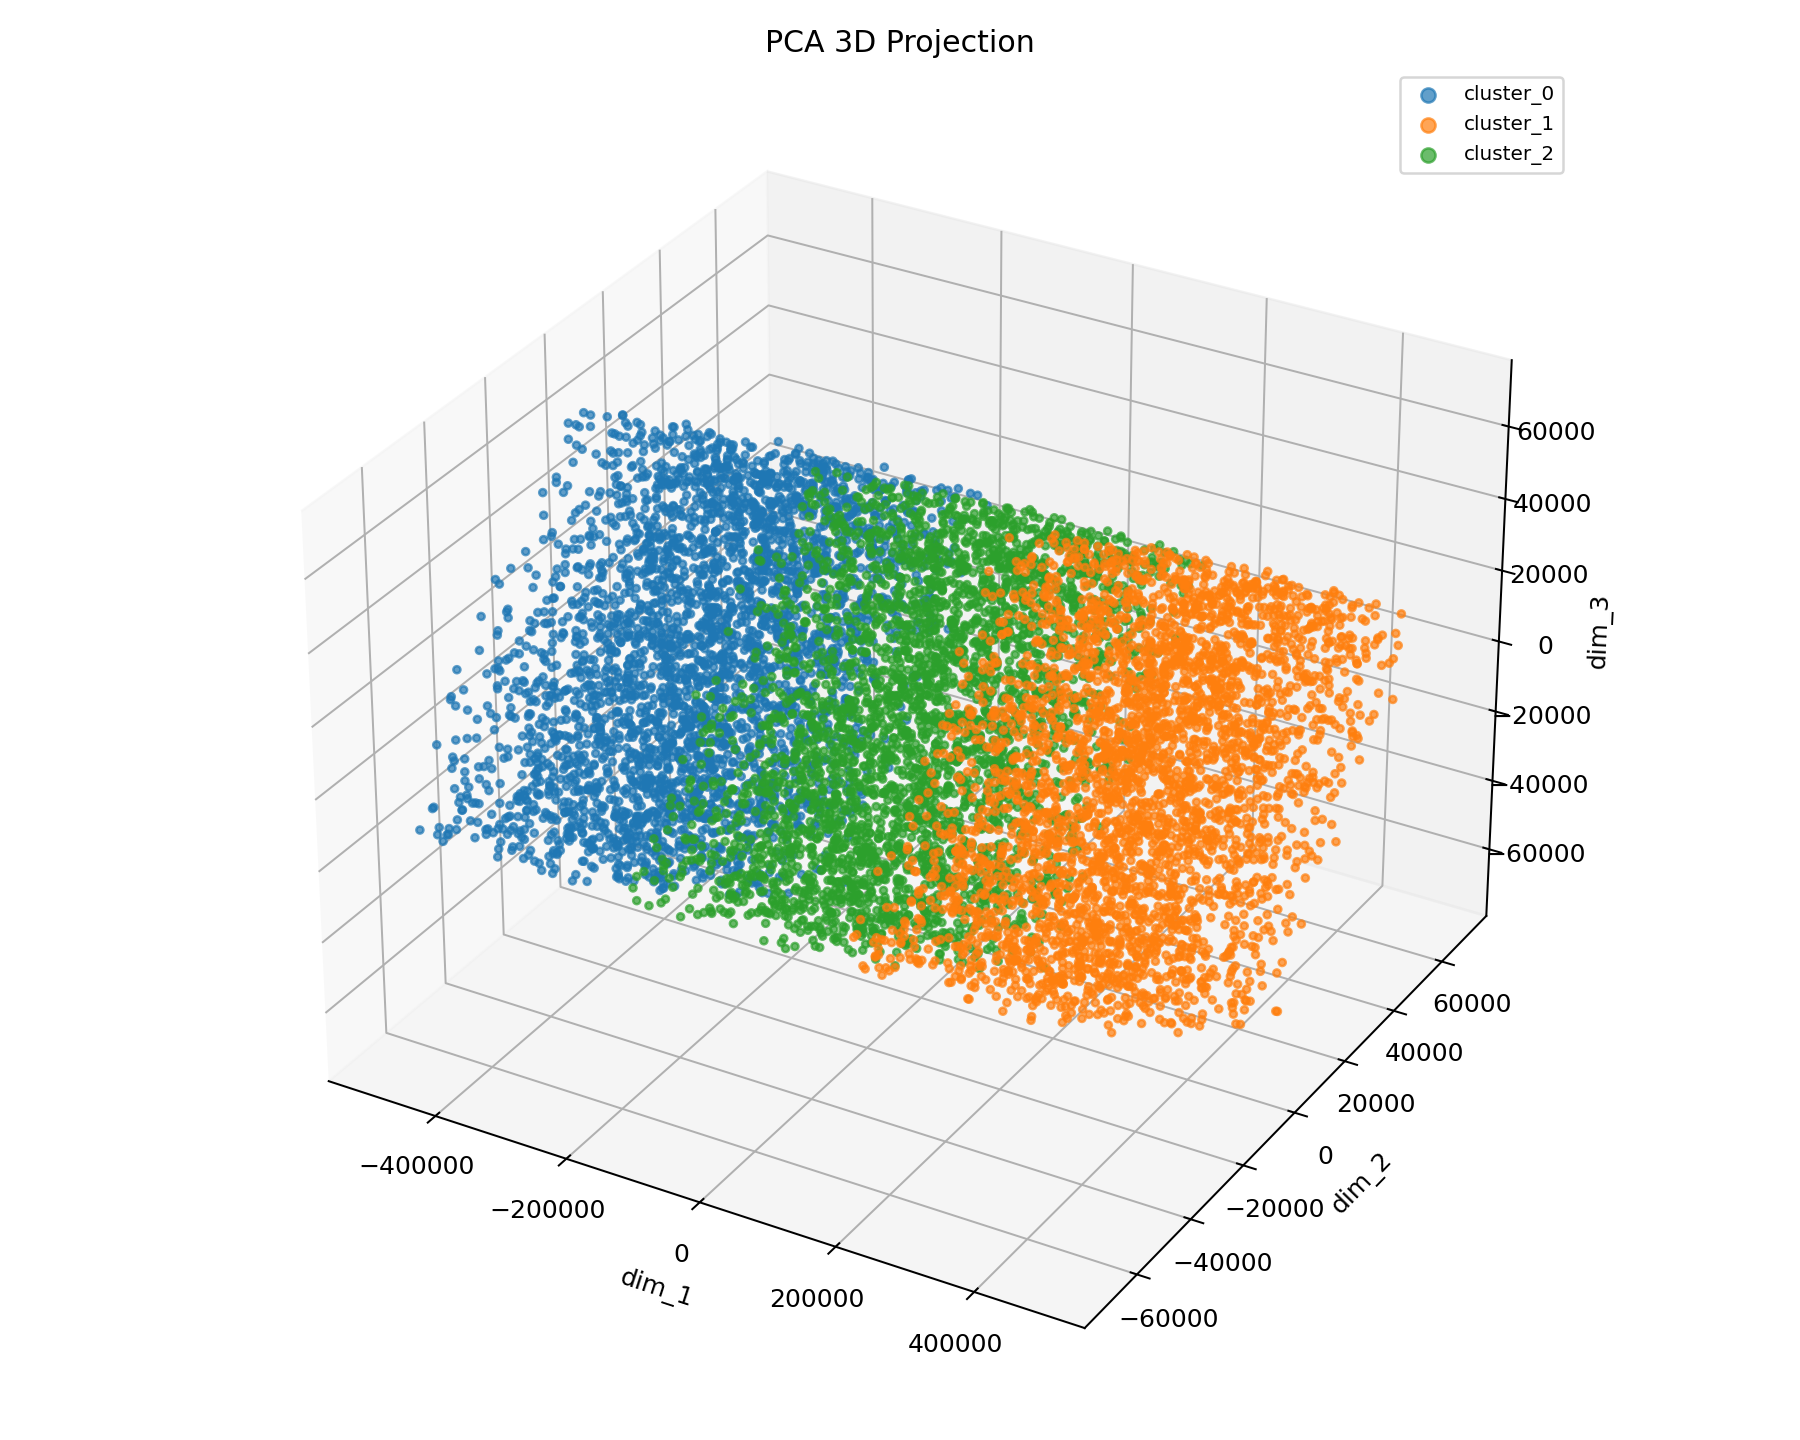
\includegraphics[width=0.48\linewidth]{task3d_viz_py/out_k3/pca_3d.png}
  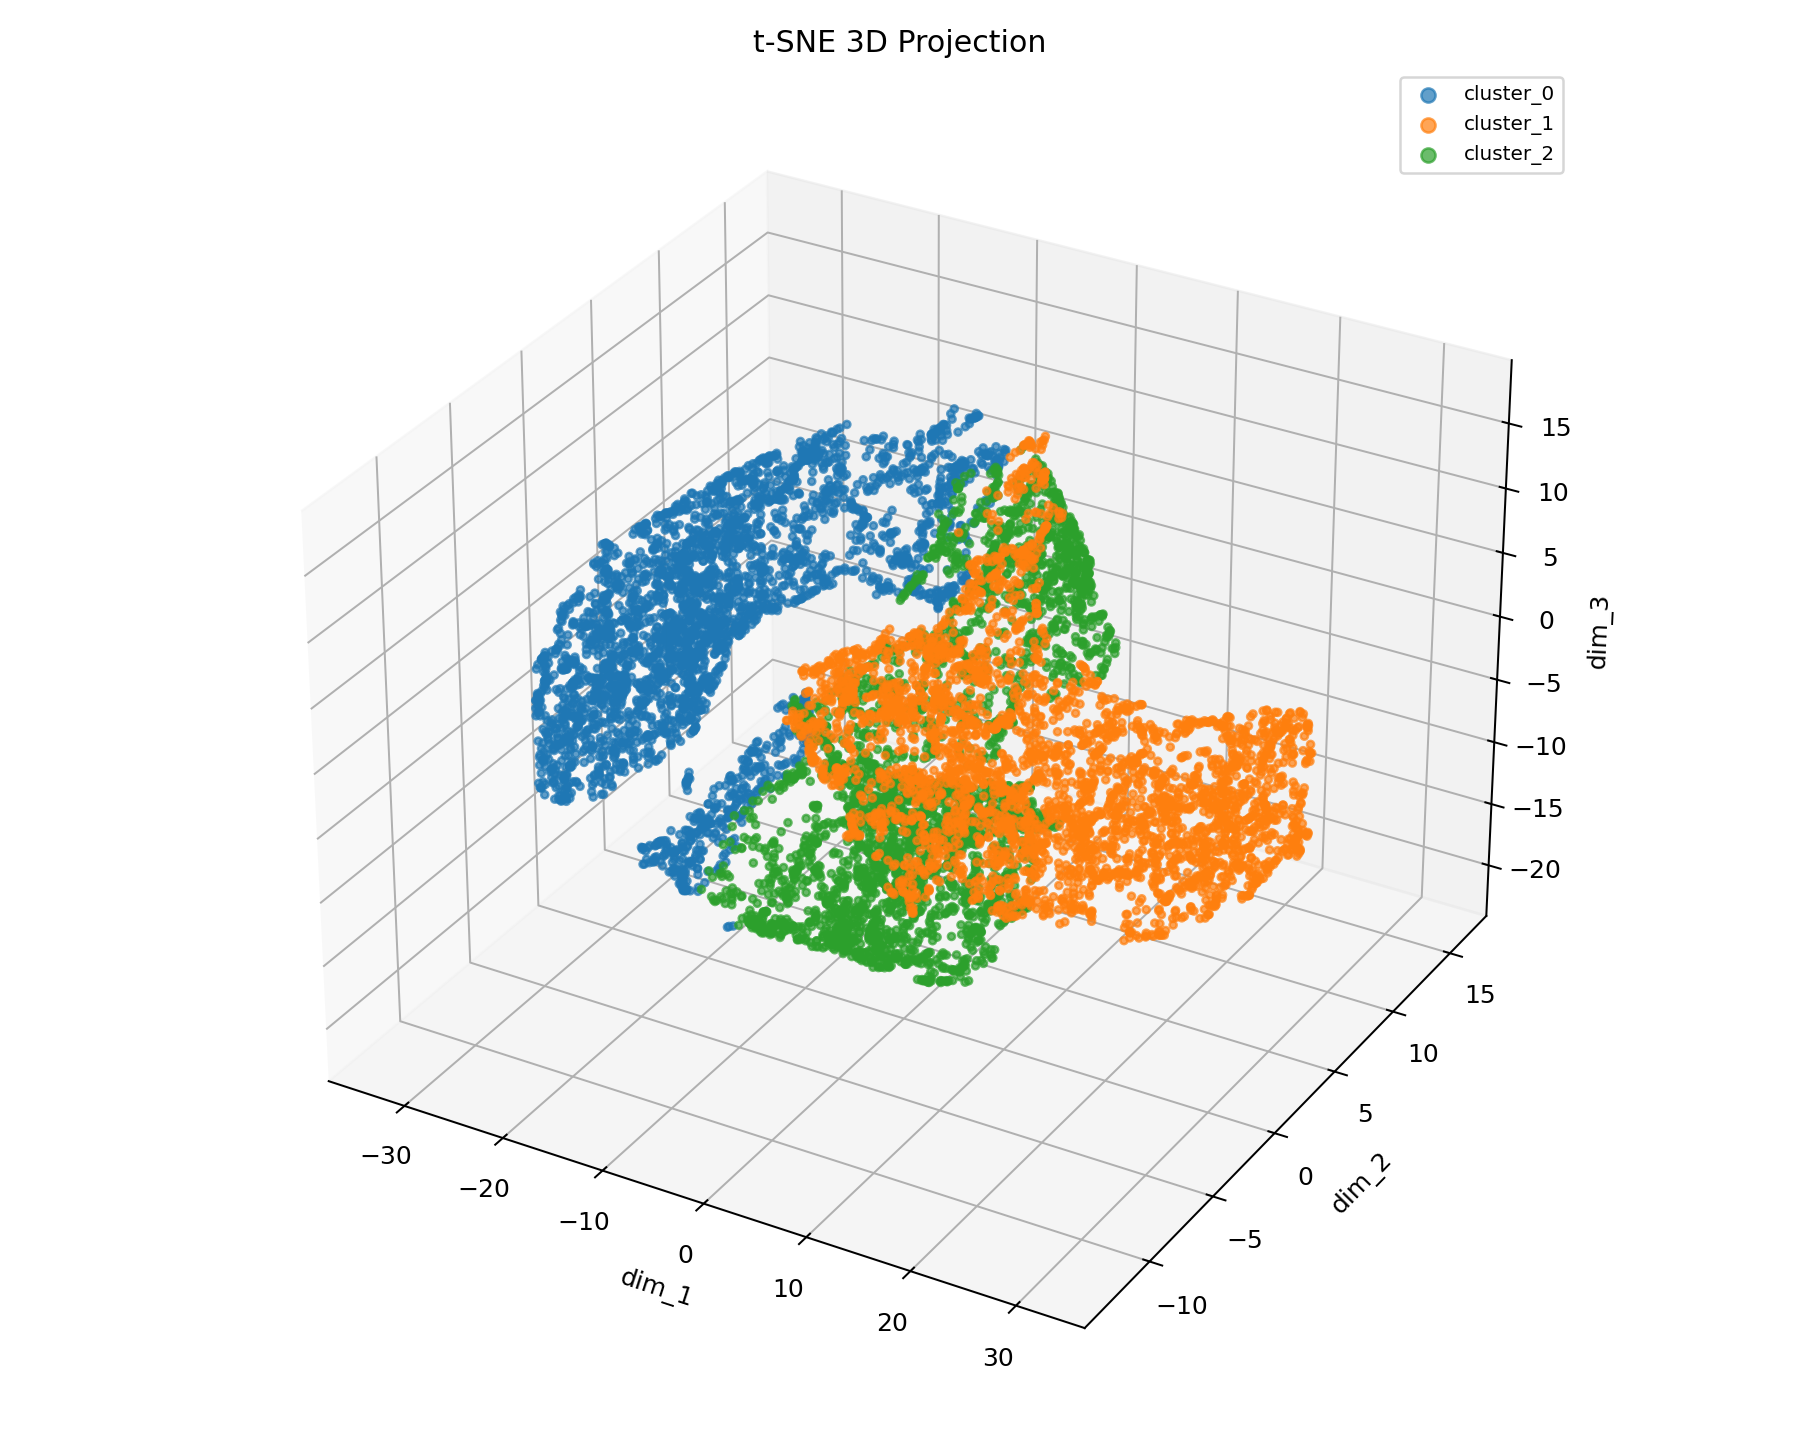
\includegraphics[width=0.48\linewidth]{task3d_viz_py/out_k3/tsne_3d.png}
  \caption{$K=3$: 3D PCA projection (left) and t-SNE projection (right) of the \textbf{Task 2 synthetic 4D dataset}, points colored by assigned cluster ID}
\end{figure}

\begin{figure}[H]
  \centering
  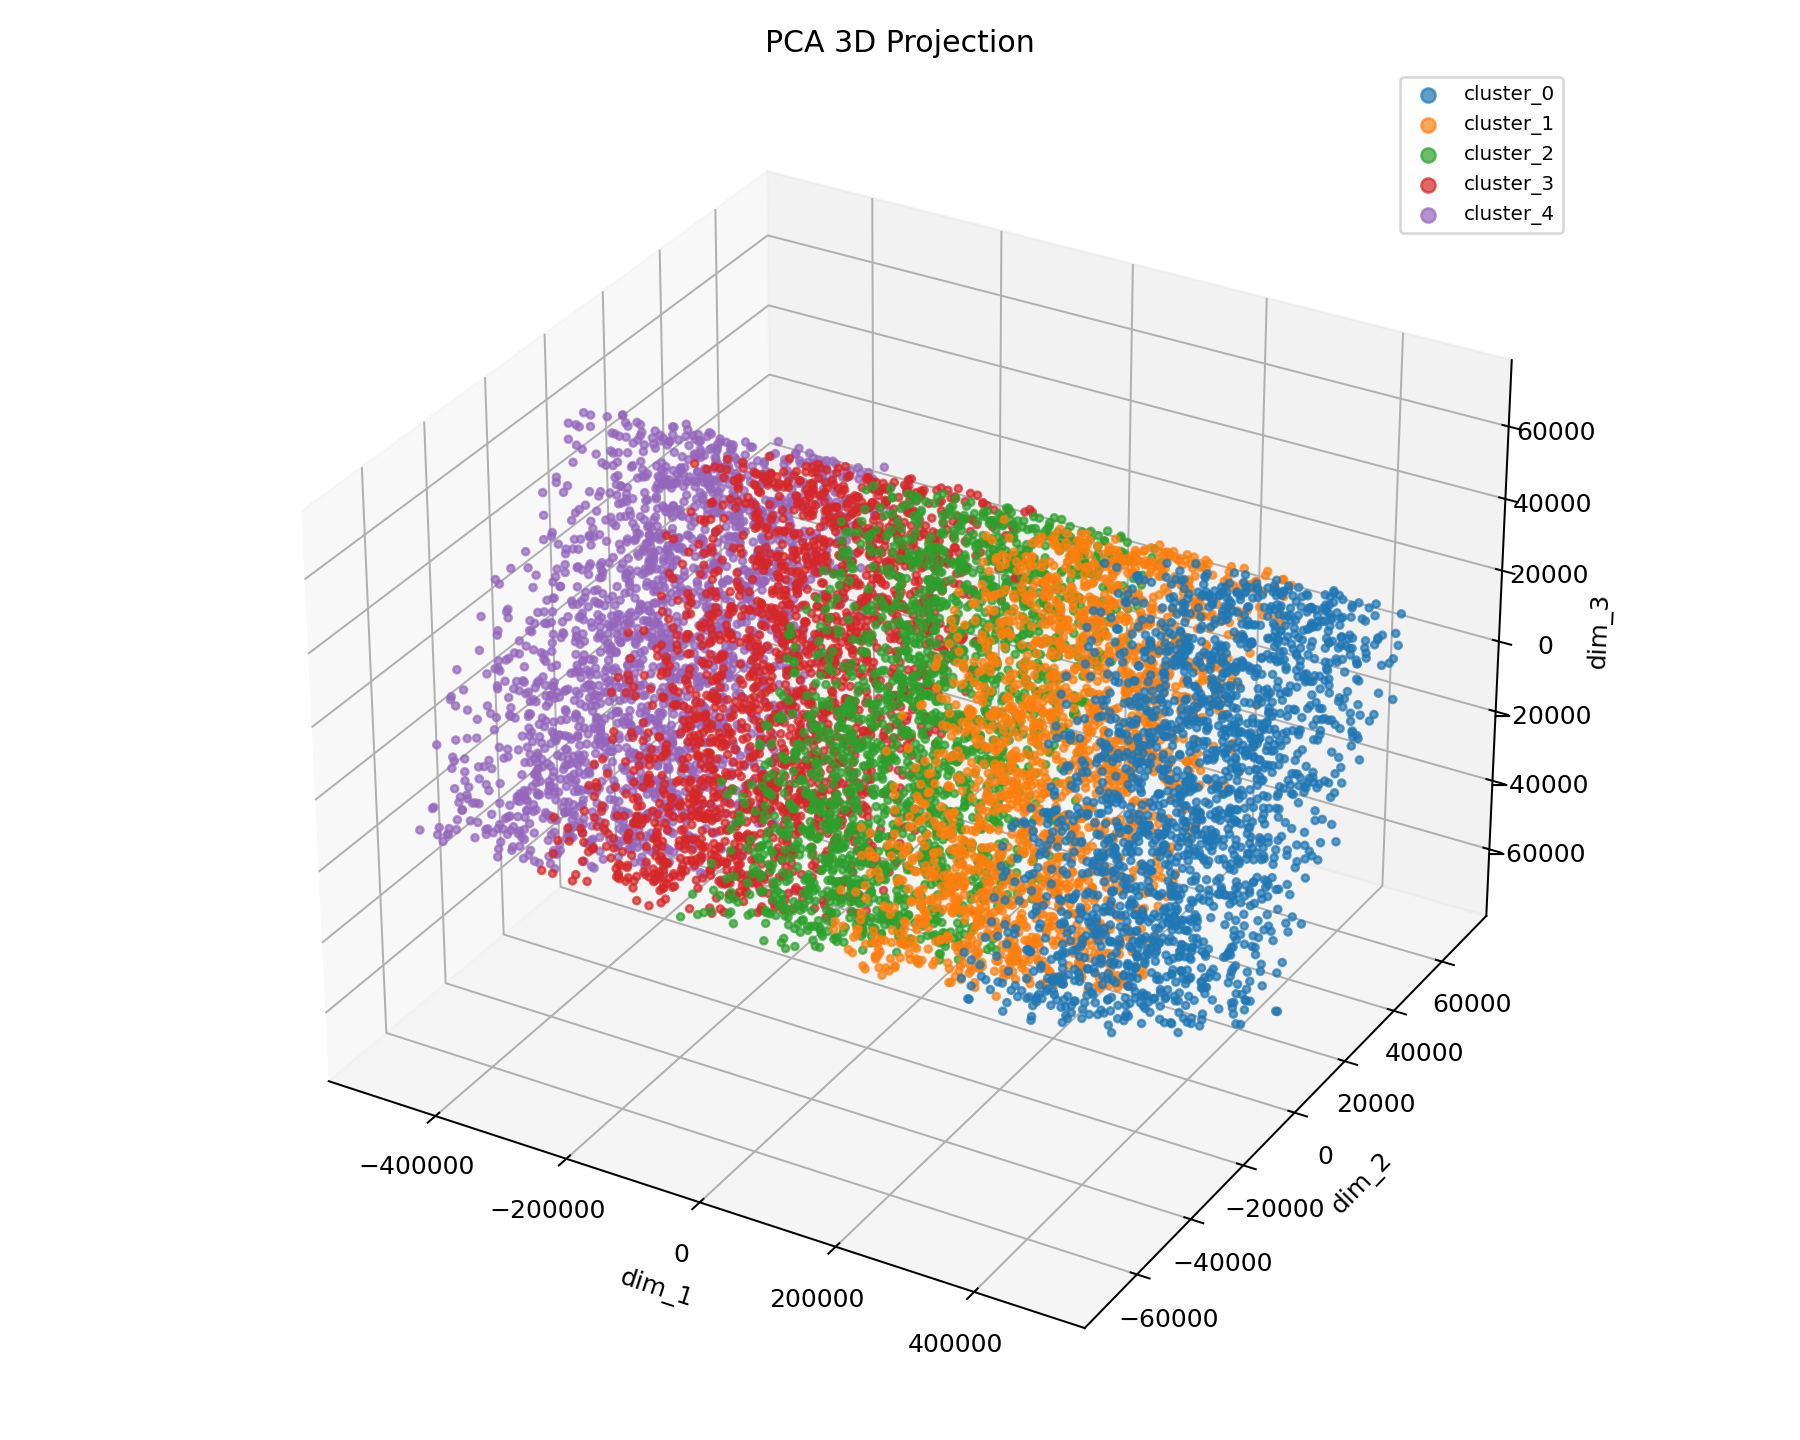
\includegraphics[width=0.48\linewidth]{task3d_viz_py/out_k5/pca_3d.png}
  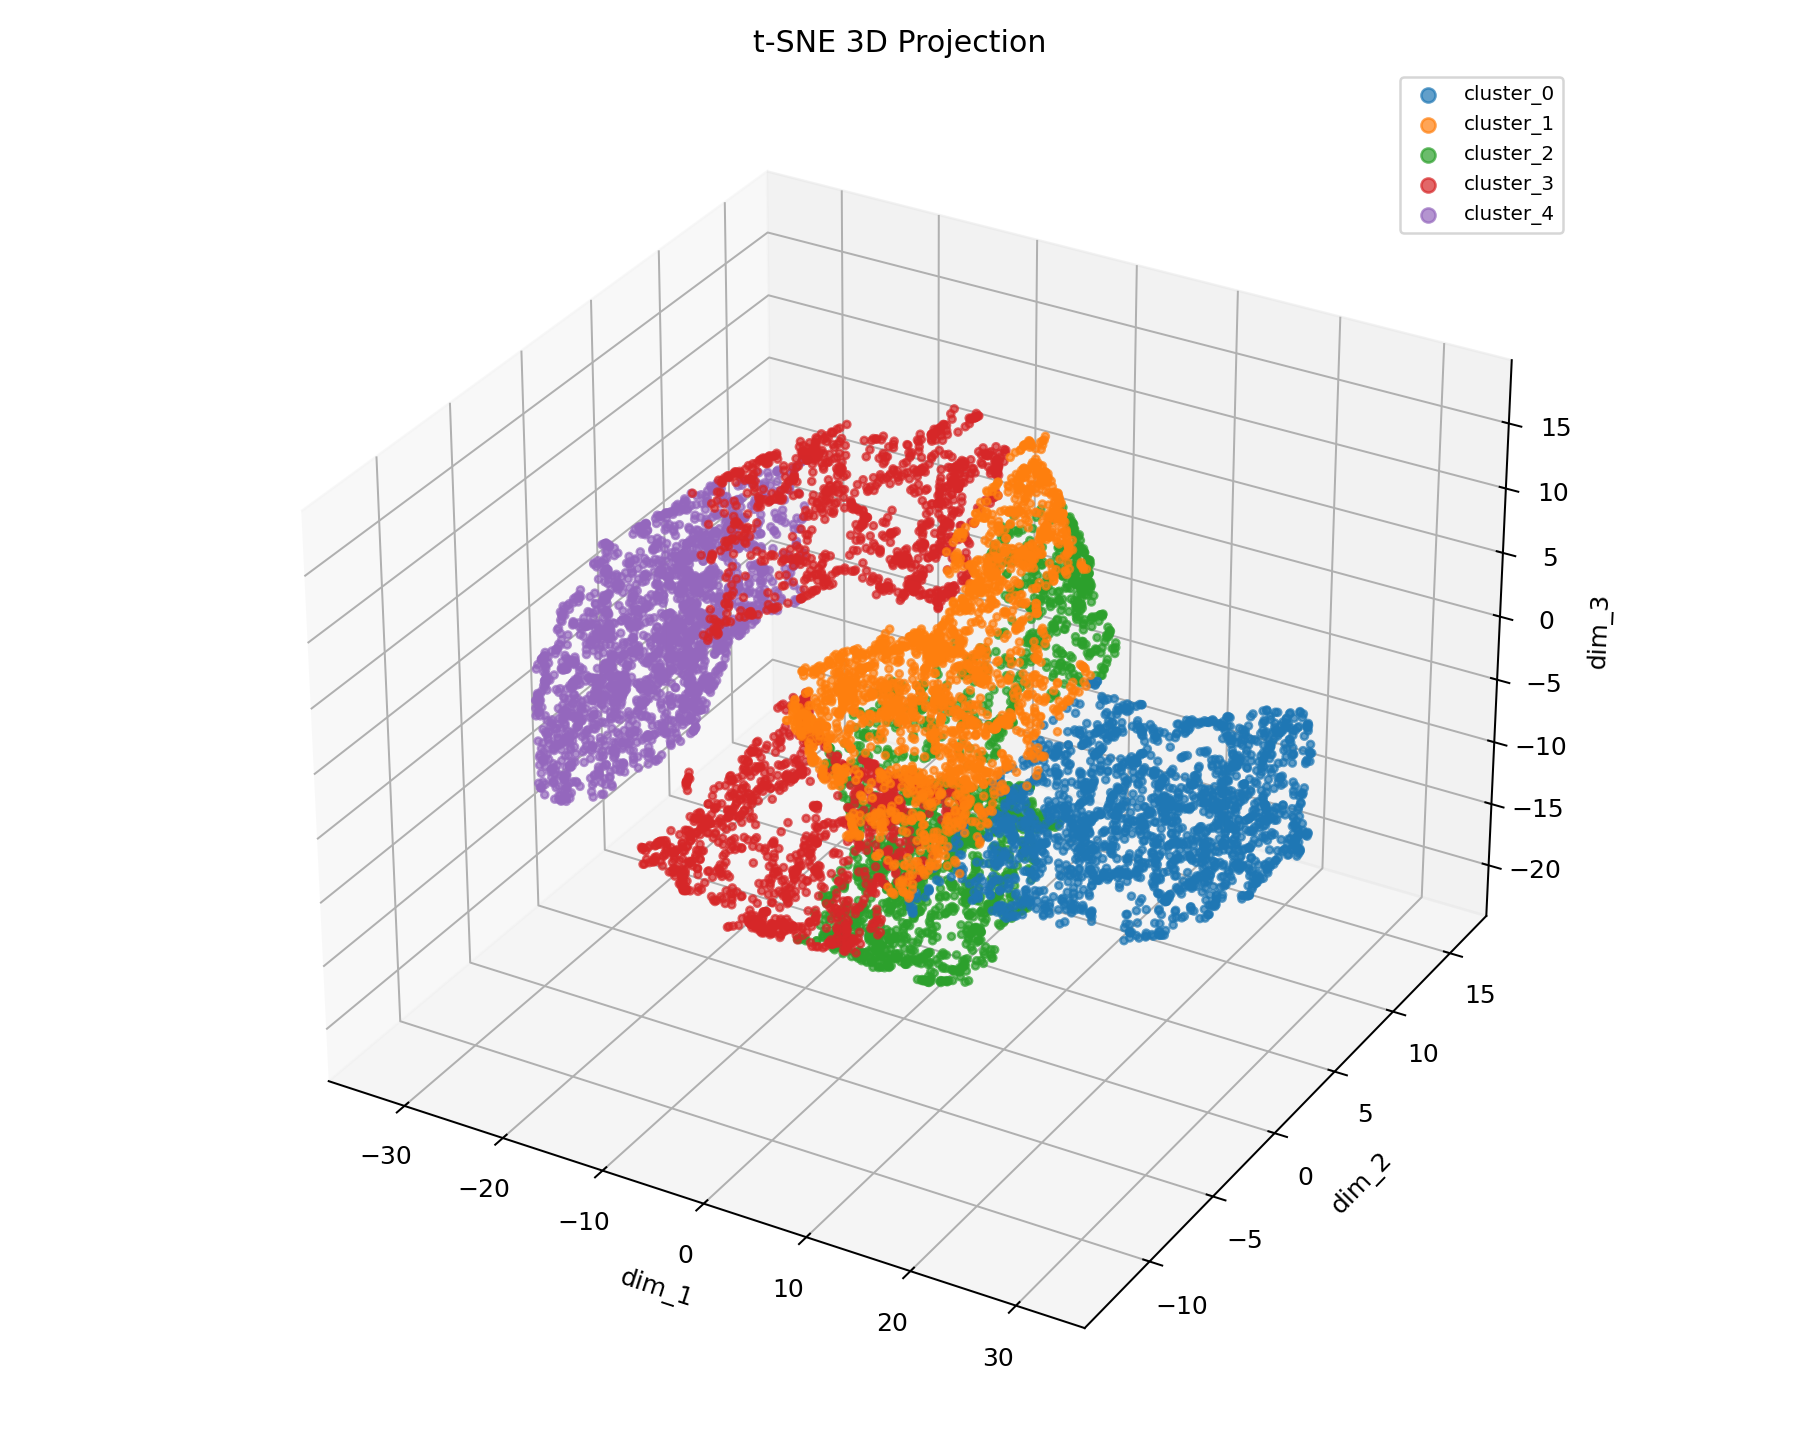
\includegraphics[width=0.48\linewidth]{task3d_viz_py/out_k5/tsne_3d.png}
  \caption{$K=5$: 3D PCA projection (left) and t-SNE projection (right) of the \textbf{Task 2 synthetic 4D dataset}, points colored by assigned cluster ID}
\end{figure}

\begin{figure}[H]
  \centering
  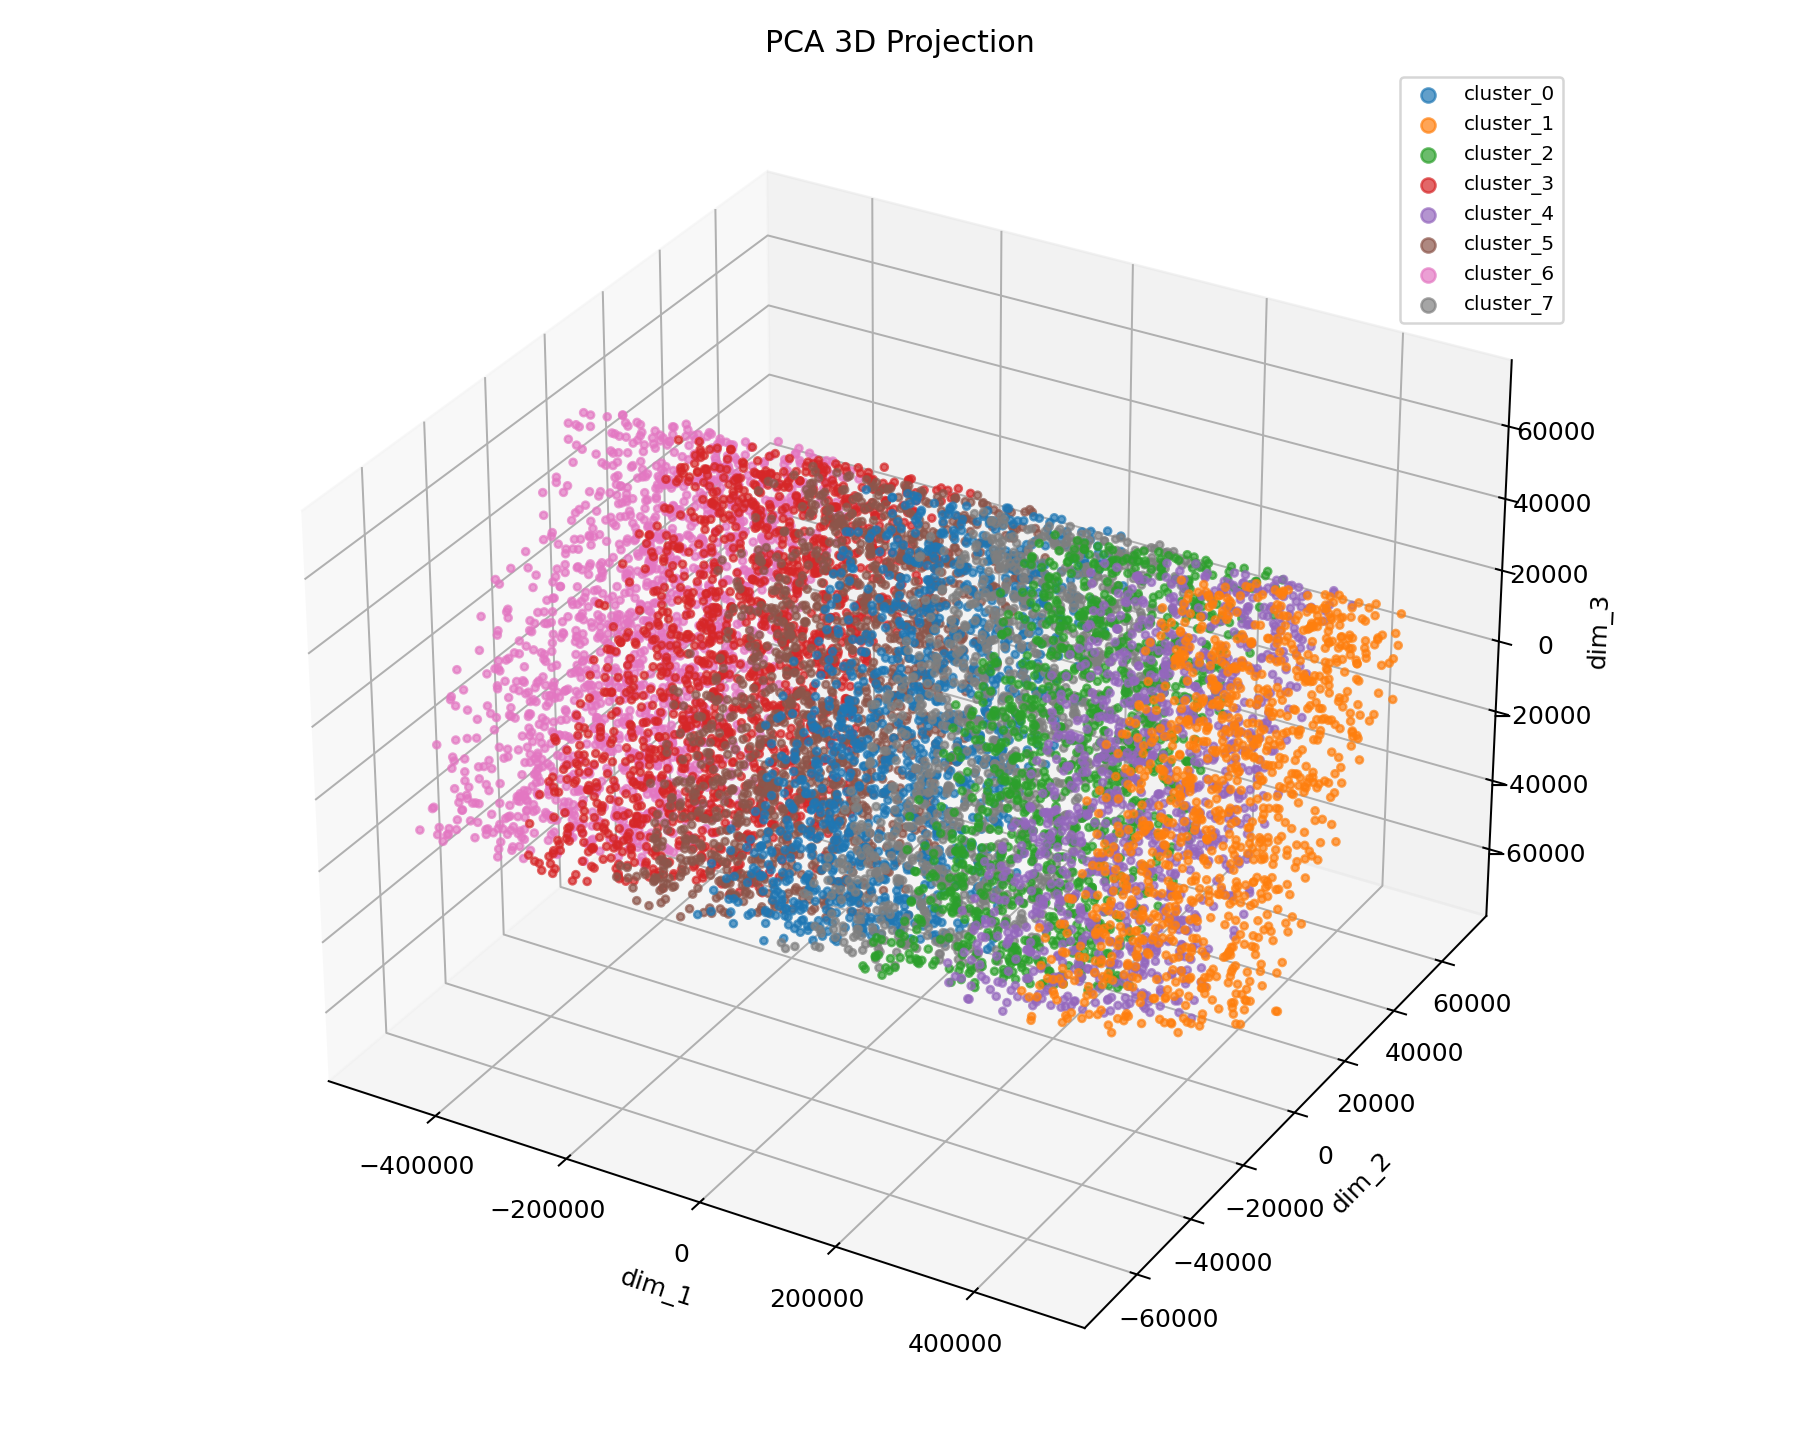
\includegraphics[width=0.48\linewidth]{task3d_viz_py/out_k8/pca_3d.png}
  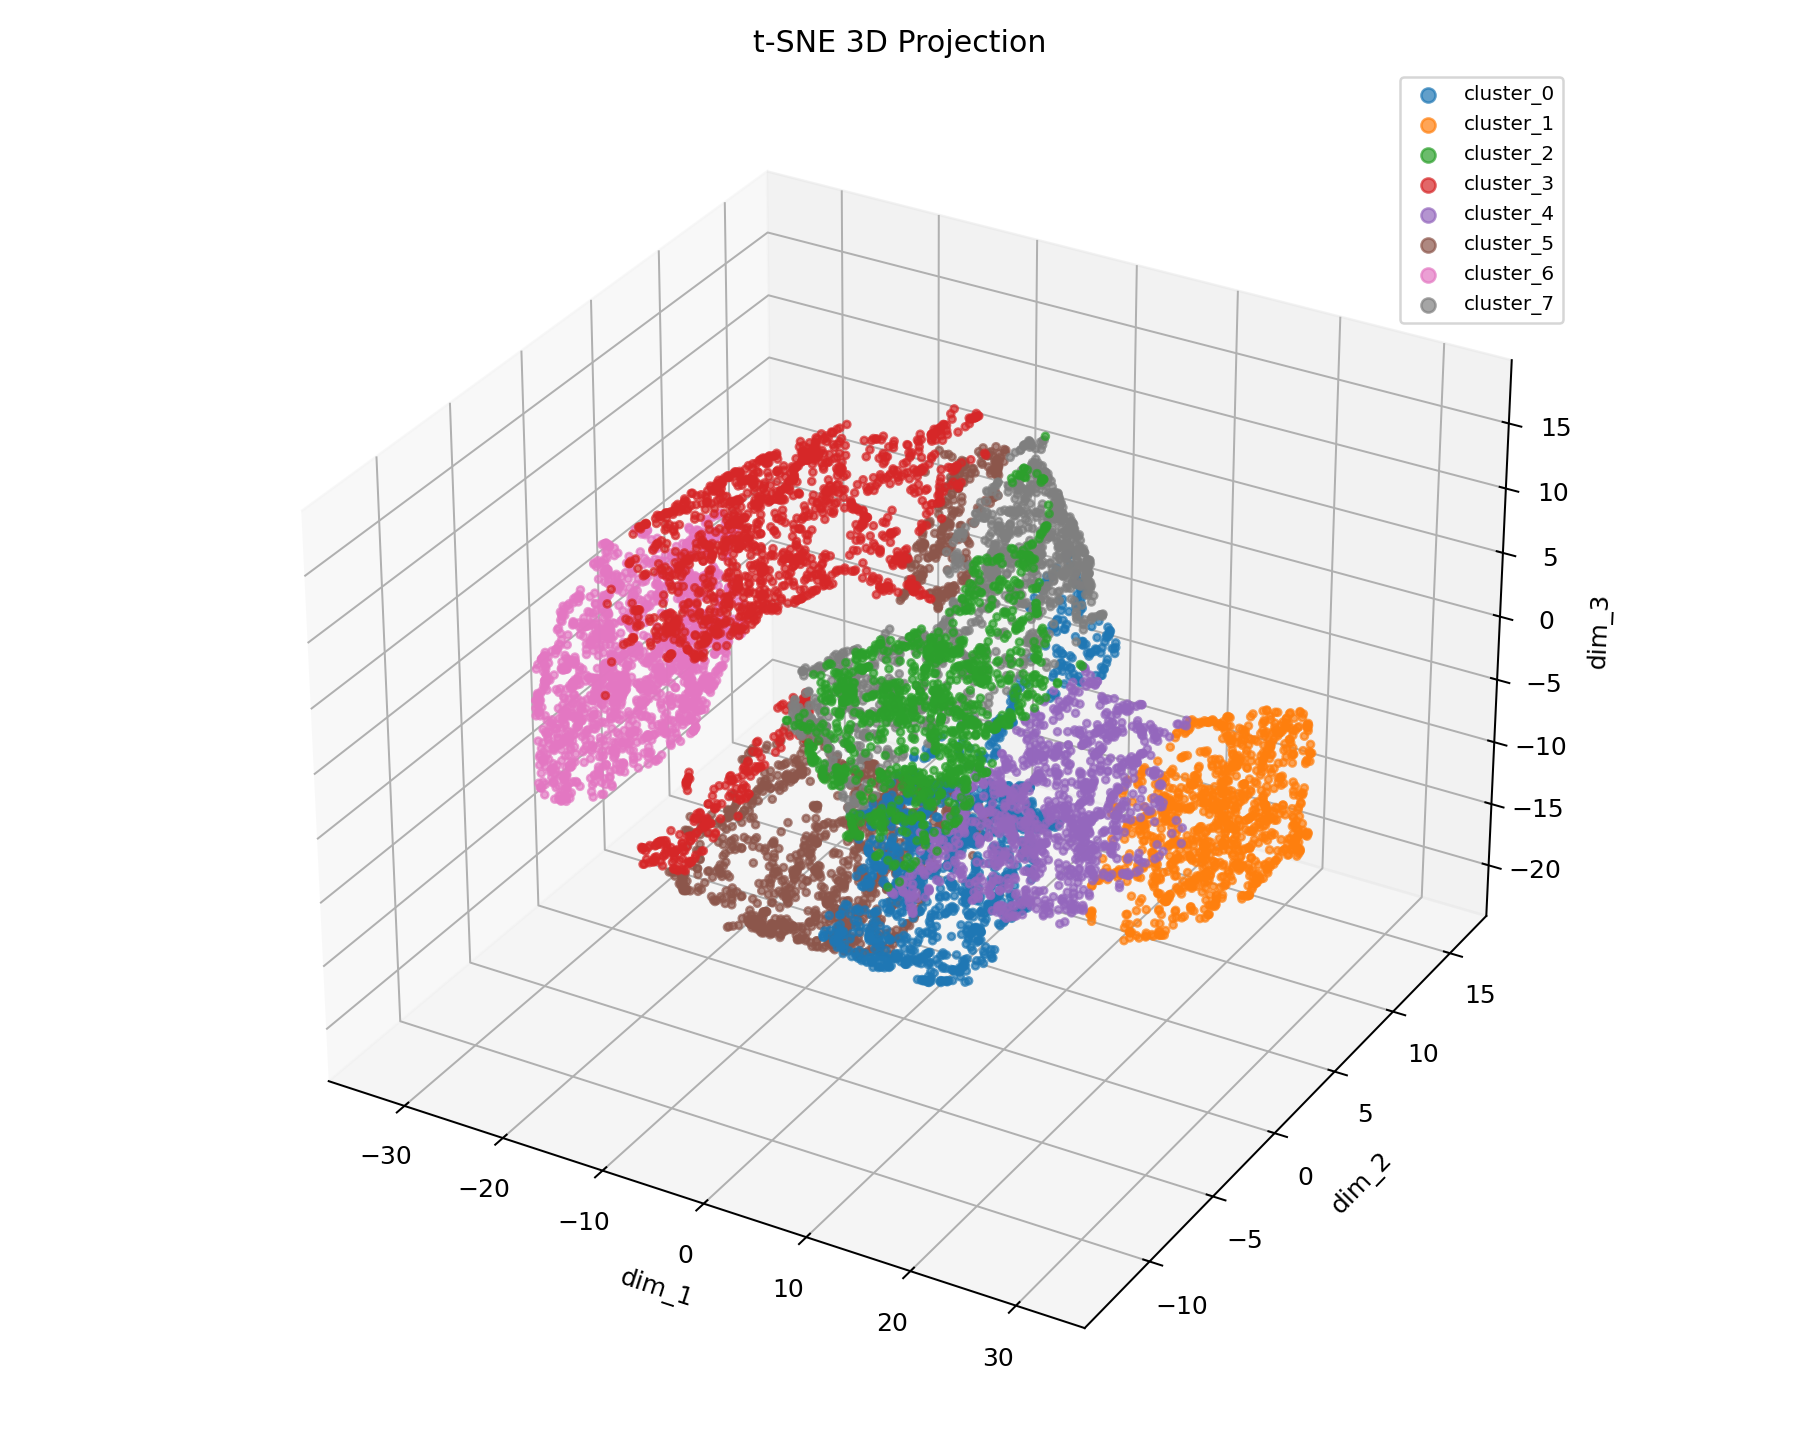
\includegraphics[width=0.48\linewidth]{task3d_viz_py/out_k8/tsne_3d.png}
  \caption{$K=8$: 3D PCA projection (left) and t-SNE projection (right) of the \textbf{Task 2 synthetic 4D dataset}, points colored by assigned cluster ID}
\end{figure}

\subsection{What We Observed}

\begin{itemize}[noitemsep,topsep=2pt]
  \item \textbf{$K=3$} gives broader, cleaner partitions clearly visible in both PCA and t-SNE projections. The three clusters span large, mostly non-overlapping regions, consistent with early convergence (round 22) and the highest SSE.
  \item \textbf{$K=5$} splits those broad regions into finer sub-groups. Boundary overlap increases in the PCA view, and the t-SNE projection reveals sub-structure that was hidden within the $K=3$ cluster regions.
  \item \textbf{$K=8$} further sub-divides the space; boundary ambiguity is highest here. Points near cluster edges are harder to assign consistently, which aligns with the observed non-convergence at $R=30$.
\end{itemize}

\begin{tcolorbox}[finding]
The visualization directly supports the SSE and convergence findings from Task 2.2(f): lower SSE at higher $K$ corresponds to finer visual partitioning, while the lack of convergence at $K=5$ and $K=8$ corresponds to the visible boundary overlap in the 3D projections. Compact clustering ($K=3$) is easier to interpret; fine-grained clustering ($K=8$) gives lower SSE at the cost of stability.
\end{tcolorbox}

% ===========================================================================
\section{Limitations}
% ===========================================================================

\begin{itemize}[noitemsep,topsep=2pt]
  \item Several runs reached the maximum round budget $R$ without satisfying the early-stop threshold ($K=5$ and $K=8$ at $R=30$). Convergence is sensitive to initialization, data distribution, and the \texttt{epsilon} setting.
  \item We kept non-converged runs in the report to show real behavior under fixed settings rather than cherry-picking results or inflating $R$.
  \item The combiner advantage was small at 10,000 points; the benefit grows substantially at larger dataset sizes where shuffle bandwidth is the dominant bottleneck.
  \item The BYOD Poker Hand dataset uses integer-valued features (suits 1--4, ranks 1--13). K-Means with Euclidean distance treats these as continuous, so cluster centers are non-integer and may not correspond to meaningful card combinations. A domain-appropriate distance metric would improve interpretability.
\end{itemize}

% ===========================================================================
\section{Team Contributions}
% ===========================================================================

{\small
\begin{longtable}{@{}p{0.17\linewidth}p{0.44\linewidth}p{0.32\linewidth}@{}}
  \rowcolor{tableheader}
  \color{white}\textbf{Member} &
  \color{white}\textbf{Implemented / Led} &
  \color{white}\textbf{Testing \& Documentation} \\
  \midrule\endhead

  \textbf{Shyam Patadia} &
  Designed and implemented the end-to-end K-Means MapReduce framework
  (\texttt{KMeansMain}) covering all five modes (SINGLE, BASIC, EARLY,
  OPT\_CENTERS, OPT\_POINTS); built the combiner and the early-termination
  convergence logic; wrote \texttt{DataSeedMain} for 4D dataset and seed
  generation; set up HDFS paths and job configuration; implemented Pig
  scripts for Tasks A, B, D, and E. &
  Executed the full K/R experiment matrix ($K\in\{3,5,8\}$,
  $R\in\{10,30\}$, both EARLY and OPT\_CENTERS modes); collected and
  validated all SSE and runtime metrics; coordinated overall report
  structure and authored the Task 2 sections. \\[6pt]

  \textbf{Nischal Patel} &
  Implemented Pig scripts for Tasks C, F, G, and H; built the Java
  visualization program (\texttt{KMeansVizMain}) for cluster-count
  extraction; wrote the Python PCA and t-SNE visualization scripts. &
  Ran the full visualization pipeline for $K\in\{3,5,8\}$ and produced all
  PCA/t-SNE plots; authored the Task 3(d) visualization section and the
  Limitations section of the report. \\[6pt]

  \rowcolor{tablealt}
  \textbf{Vansh Patel} &
  Contributed to Task 1 Pig implementation and supported the Task 3(a)
  BYOD pipeline. &
  Assisted with experiment runs and report review. \\

\end{longtable}
\normalsize}

\end{document}
